\documentclass[11pt]{article}
\usepackage{graphicx}
\usepackage{setspace}
\usepackage{extsizes}
\usepackage{float}
\usepackage{amsmath, amsthm, amssymb}

\usepackage[left=1cm, right=1cm, top=.25cm, bottom=.5cm]{geometry}
\pagenumbering{gobble}


\title{Problem Set 3}
\author{\vspace{-2.0cm}Joanne Wardell}
\date{9 May 2019}

\begin{document}
\maketitle

\begin{center}
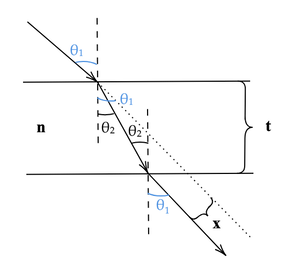
\includegraphics{pic2.png}
\end{center}

Show that the displacement $x$ of an emerging light ray
$x = \frac{t\sin{\theta_{1}-\theta_{2}}}{\cos{\theta_{2}}}$
can be approximated as 
$\frac{t\theta(n-1)}{n}$
assuming that the incident ray is paraxial.


\[\frac{t\sin{\theta_{1}-\theta_{2}}}{\cos{\theta_{2}}}\]\\
\[\frac{t(\sin{\theta_{1}}\cos{\theta_{2}}-\cos{\theta_{1}}\sin{\theta_{2}})}{\cos{\theta_{2}}}\]\\
\[\frac{t(\theta_{1}\cos{\theta_{2}}-\theta_{2}\cos{\theta_{1}})}{\cos{\theta_{2}}} \text{\footnotesize{     by paraxial ray approximation}}\]\\
\[\frac{t\theta(\cos{\theta_{2}}-\cos{\theta_{1}})}{\cos{\theta_{2}}}\]\\
\[t\theta(\frac{\cos{\theta_{2}}}{\cos{\theta_{2}}}-\frac{\cos{\theta_{1}}}{\cos{\theta_{2}}})\]\\
\[t\theta(\frac{n}{n}-\frac{1}{n}) \text{\footnotesize{     by Snell's law}}\]\\
\[\frac{t\theta(n-1)}{n}\]



\end{document}

